% !TEX encoding = UTF-8 Unicode
%!TEX root = thesis.tex
% !TEX spellcheck = en-US
%%=========================================
\chapter{Visualization}

%%=========================================
\section{Prototype} % (fold)
\label{sub:prototype}
After problem analyzing and related approach investigation, below are the summarized criteria for this project:
\begin{itemize}
	\item Display both general and detailed information of matching results
	\item Ontology navigation, exploration and searching
	\item Intuitive display for large ontology
	\item Ability to reveal the difference between matching algorithms
	\item User feedback acquisition
\end{itemize}

Based on the criteria above, we developed the prototype in the first stage. 

The main principle of this design is for large ontology, we have to reduce the amount of data every time we represent information to users. In other word, we need to present the most valuable data within a certain size. So we consider to provide general processed information instead of raw results. Further more, consider that users do not need so much information at one time, we show the results level by level. As long as navigation and searching functions are available, users can easily locate any single ontology node in the whole structure and see the result they need.

The information we use here is the matching similarity confidence, represented by a pie chart. The reason of using the pie chart is that, no matter how large the data size is, the pie chart requires only a small area. In addition, this feature proved to be an advantage then comparing performances of different algorithms.

\begin{figure}[htb]
	\centering
	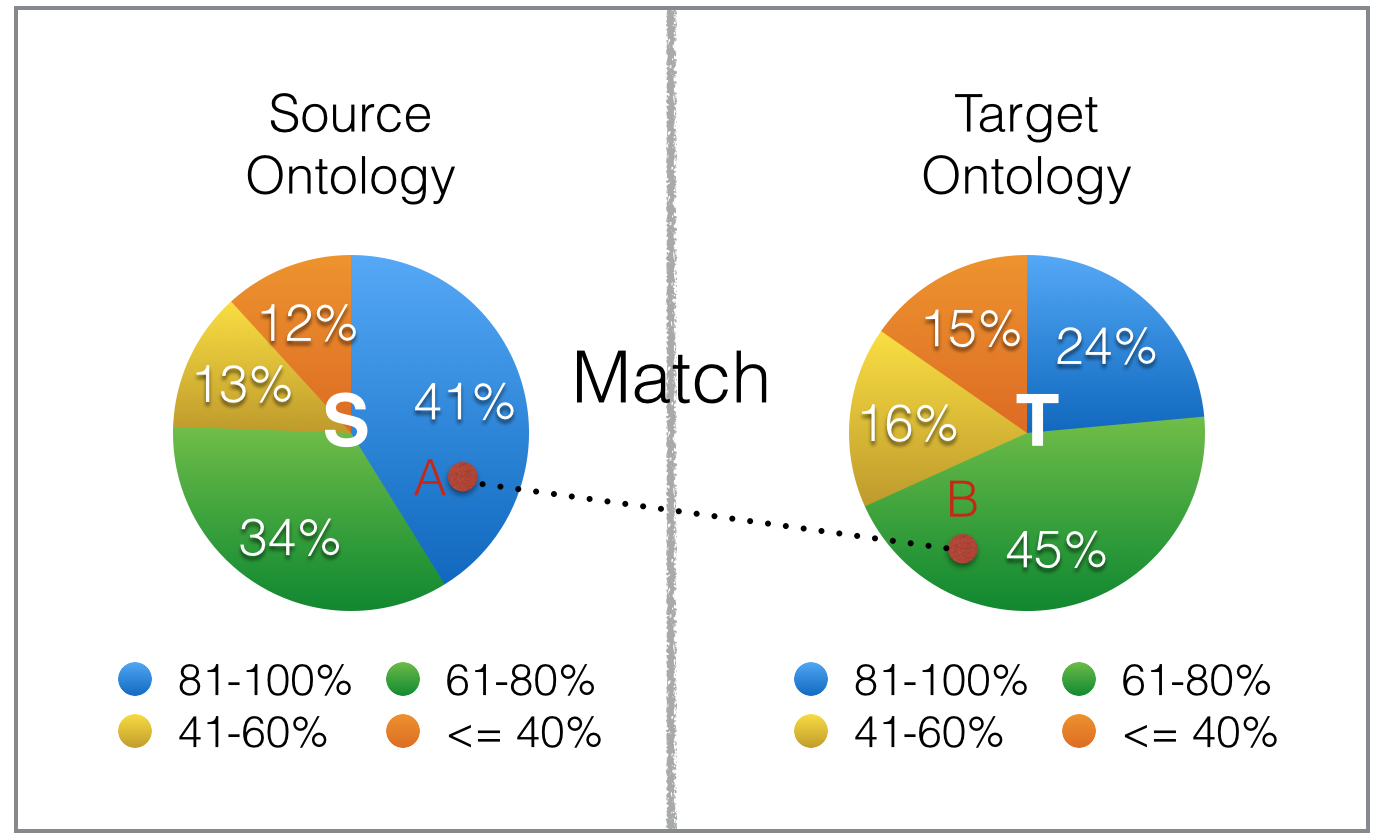
\includegraphics[width=3.5in]{pics/proto_pie.png}
	\caption{Prototype mathcing result interface}
	\label{fig:proto_pie}
\end{figure}
	
As shown in Fig.\ref{fig:proto_pie}, we divide the similarity into different ranges. For a certain source node $S$, we show the percentage of its children's matching confidence that fall in the corresponding range. In the right pie chart, matched target node $T$ of $S$ shows its children's matching results in the same way. 

\begin{figure}[htb]
	\centering
	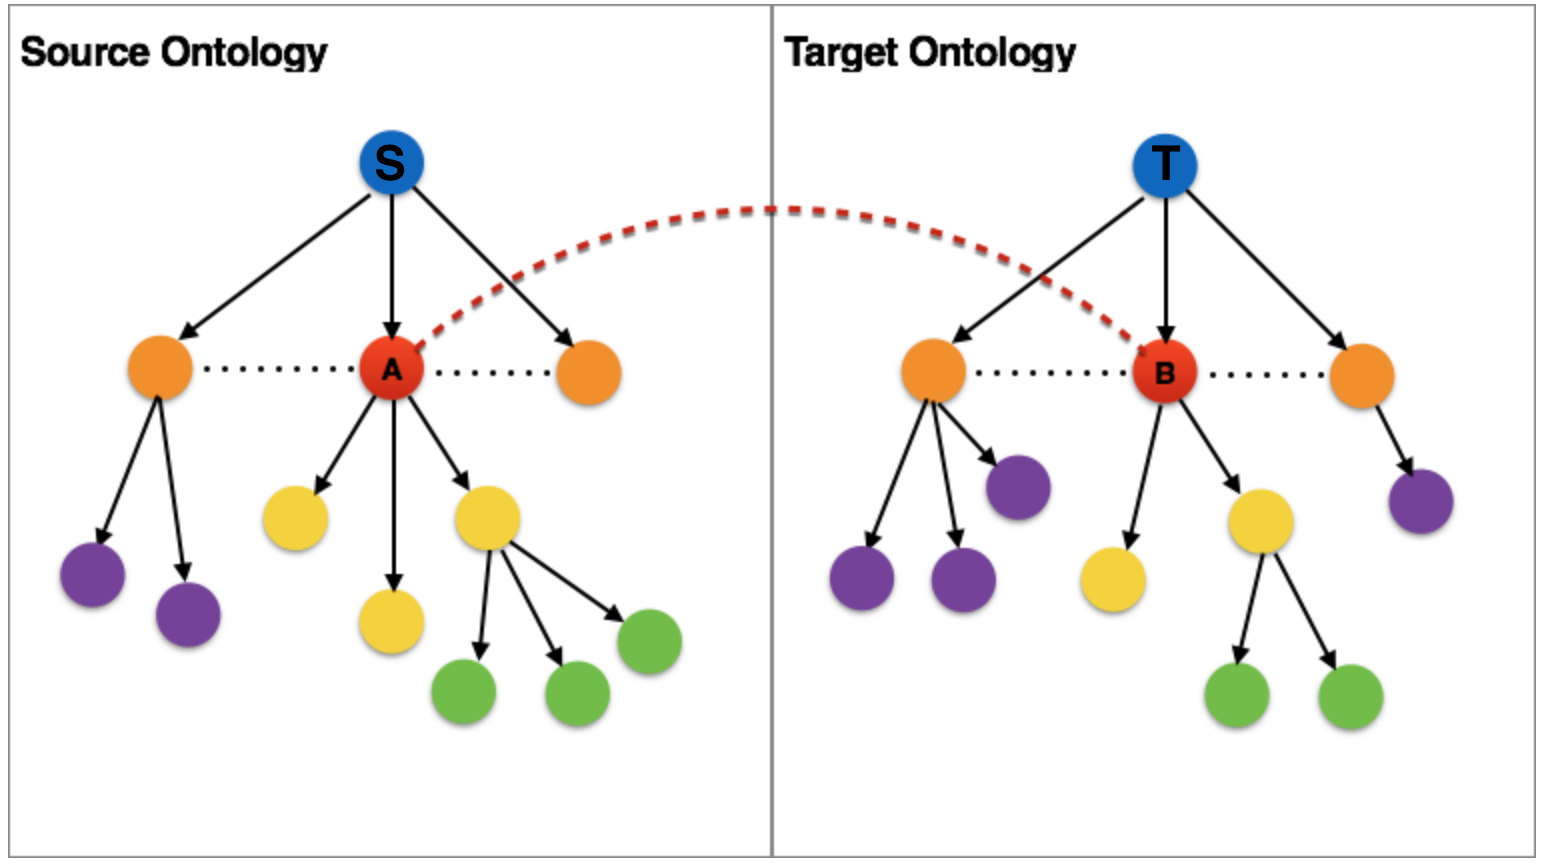
\includegraphics[width=3.5in]{pics/proto_tree.png}
	\caption{Prototype structure interface}
	\label{fig:proto_tree}
\end{figure}

Besides the general information, we also provide detailed information about matching results and ontology structures. To deal with large ontology, we make use of the fact that users tend to pay more attention to structure-close ontology. So we only show the parent, children and siblings of the current node in view. This is clearly illustrated by Fig.\ref{fig:proto_tree}.

The next question is how to combine the general and detailed view together. In order to let users easily see both two views, we provide a list represents the children in range and a treeview represents the siblings of the current node. 

\begin{figure*}[!ht]
	\centering
	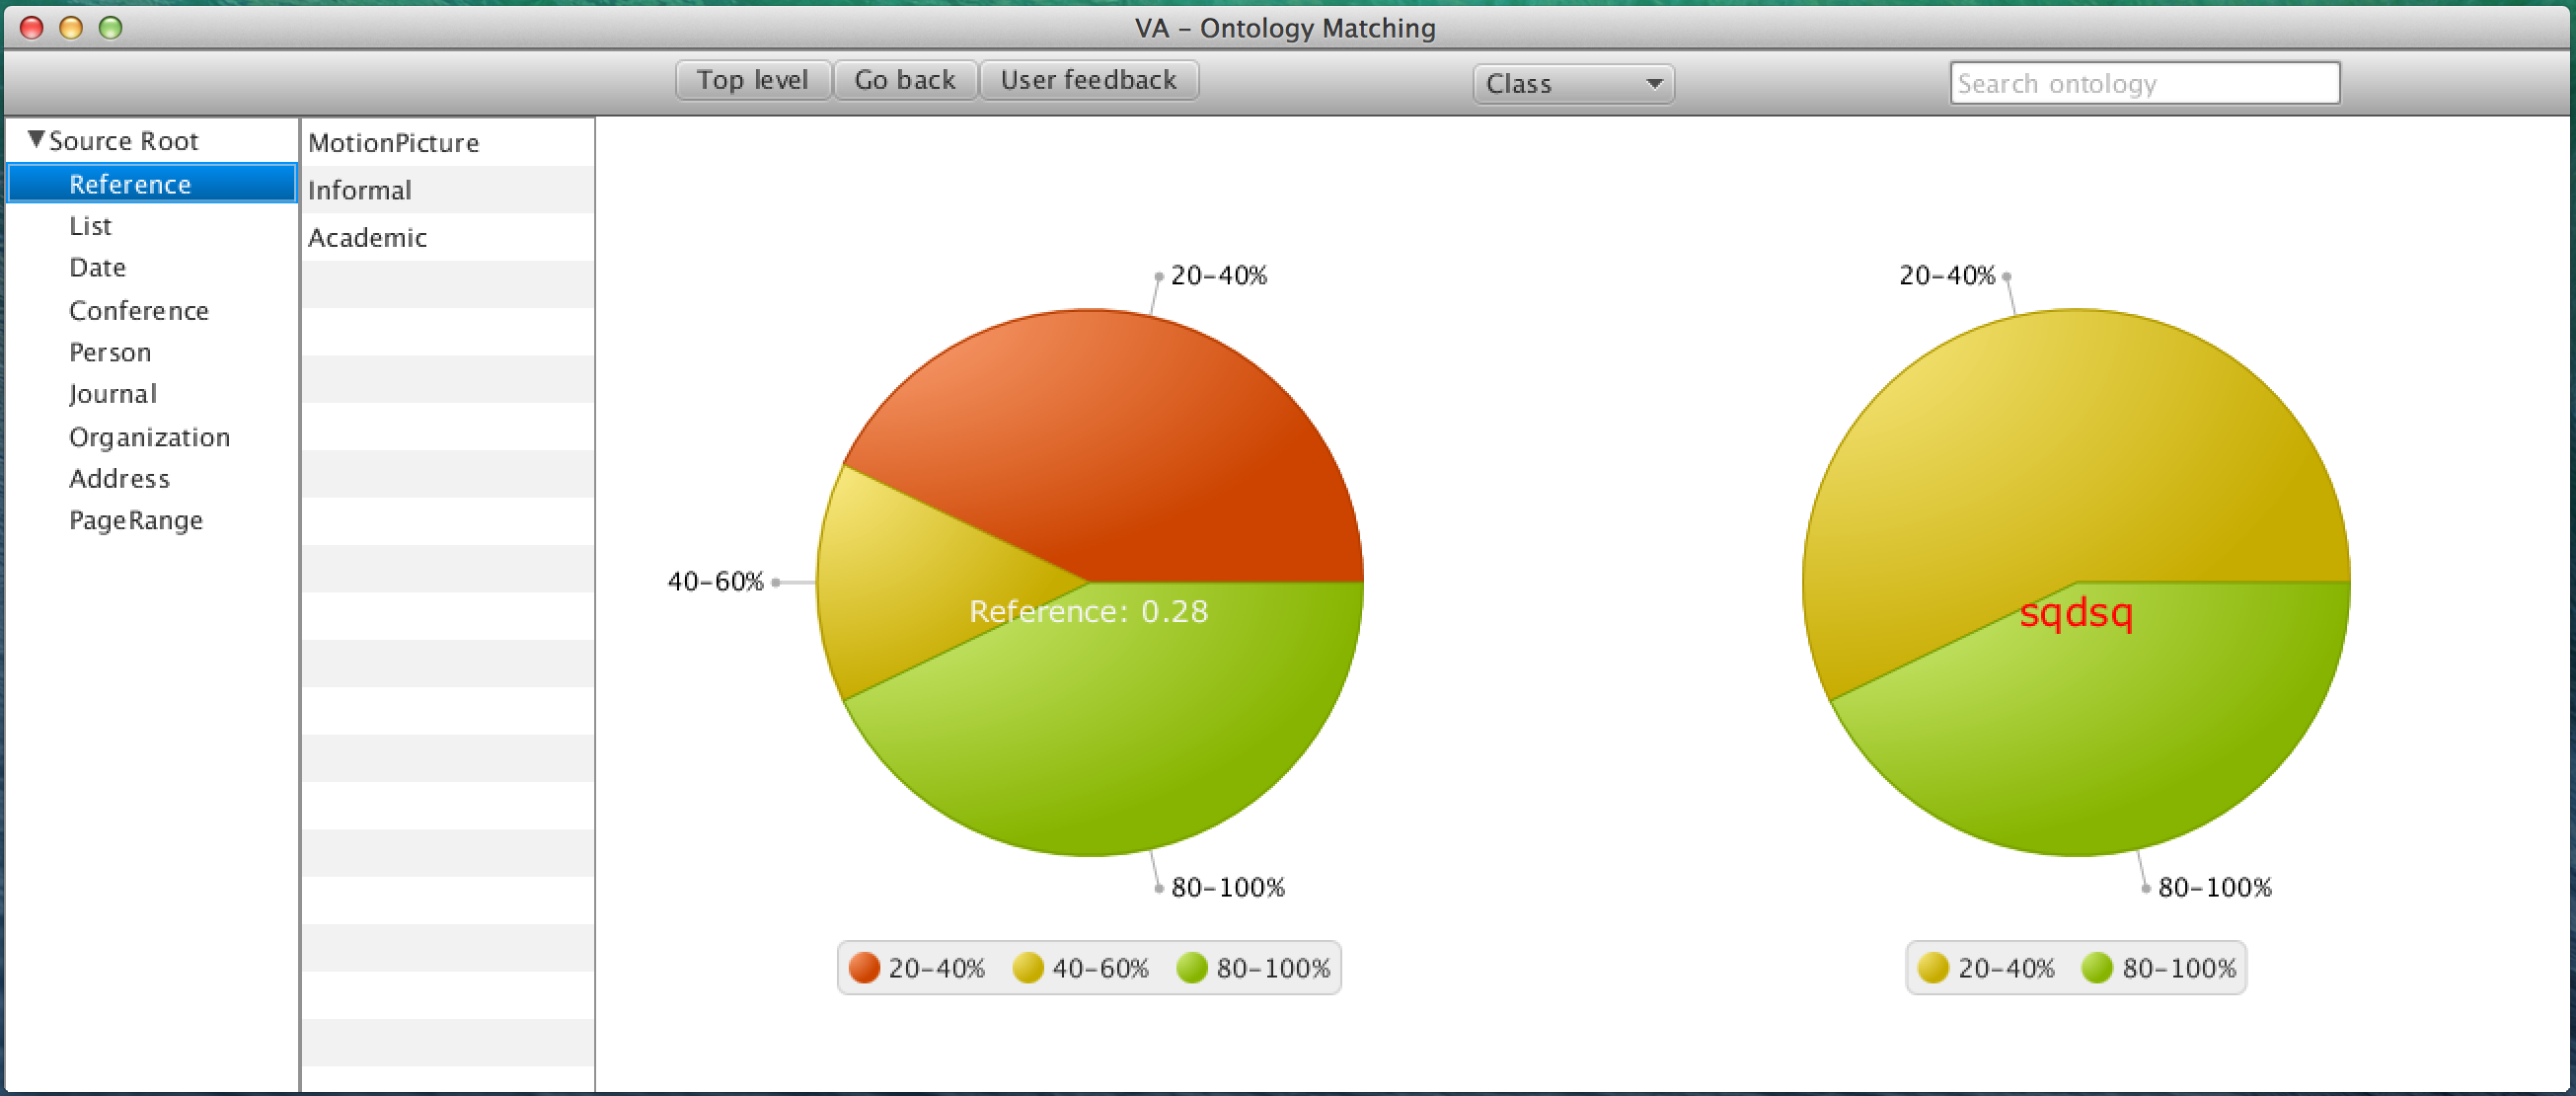
\includegraphics[width=6.5in]{pics/gui.png}
	\caption{Main panel}
	\label{fig:main_panel}
\end{figure*}
Based on the prototype we developed the first version of this application which is shown in Fig.\ref{fig:main_panel}.

%%=========================================
\section{Application Workflow}
\label{sub:application_work_flow}
Fig.\ref{fig:main_panel} shows the major user interface of this application. Same as the prototype we discussed above, in the center area there are two pie charts, representing the matching result distribution of source and target ontology separately. 

Left to the pie charts there is a list. When users click on a pie chart slice, it shows the matching ontology nodes with matching confidence falling in the sliced area, ordered by similarity confidence. Clicking on a node in the list leads to an update of the pie charts. The leftmost part is a tree view. It shows all siblings of the current node. When clicking on a node in the tree view, both the pie charts and the lists will be updated. On the top right there is a search box. When entering the name of the node and press enter key on the keyboard, the left pie chart will show the target node and everything on the panel will be updated correspondingly. Last but not the least, for better navigation we provide additional functions such as ``go to the top level'', ``go to the previous level'' and ``switching between class and property''.

To view the application workflow please see Fig.\ref{fig:workflow}
%[need more detail here?]

\begin{figure*}[!ht]
	\centering
	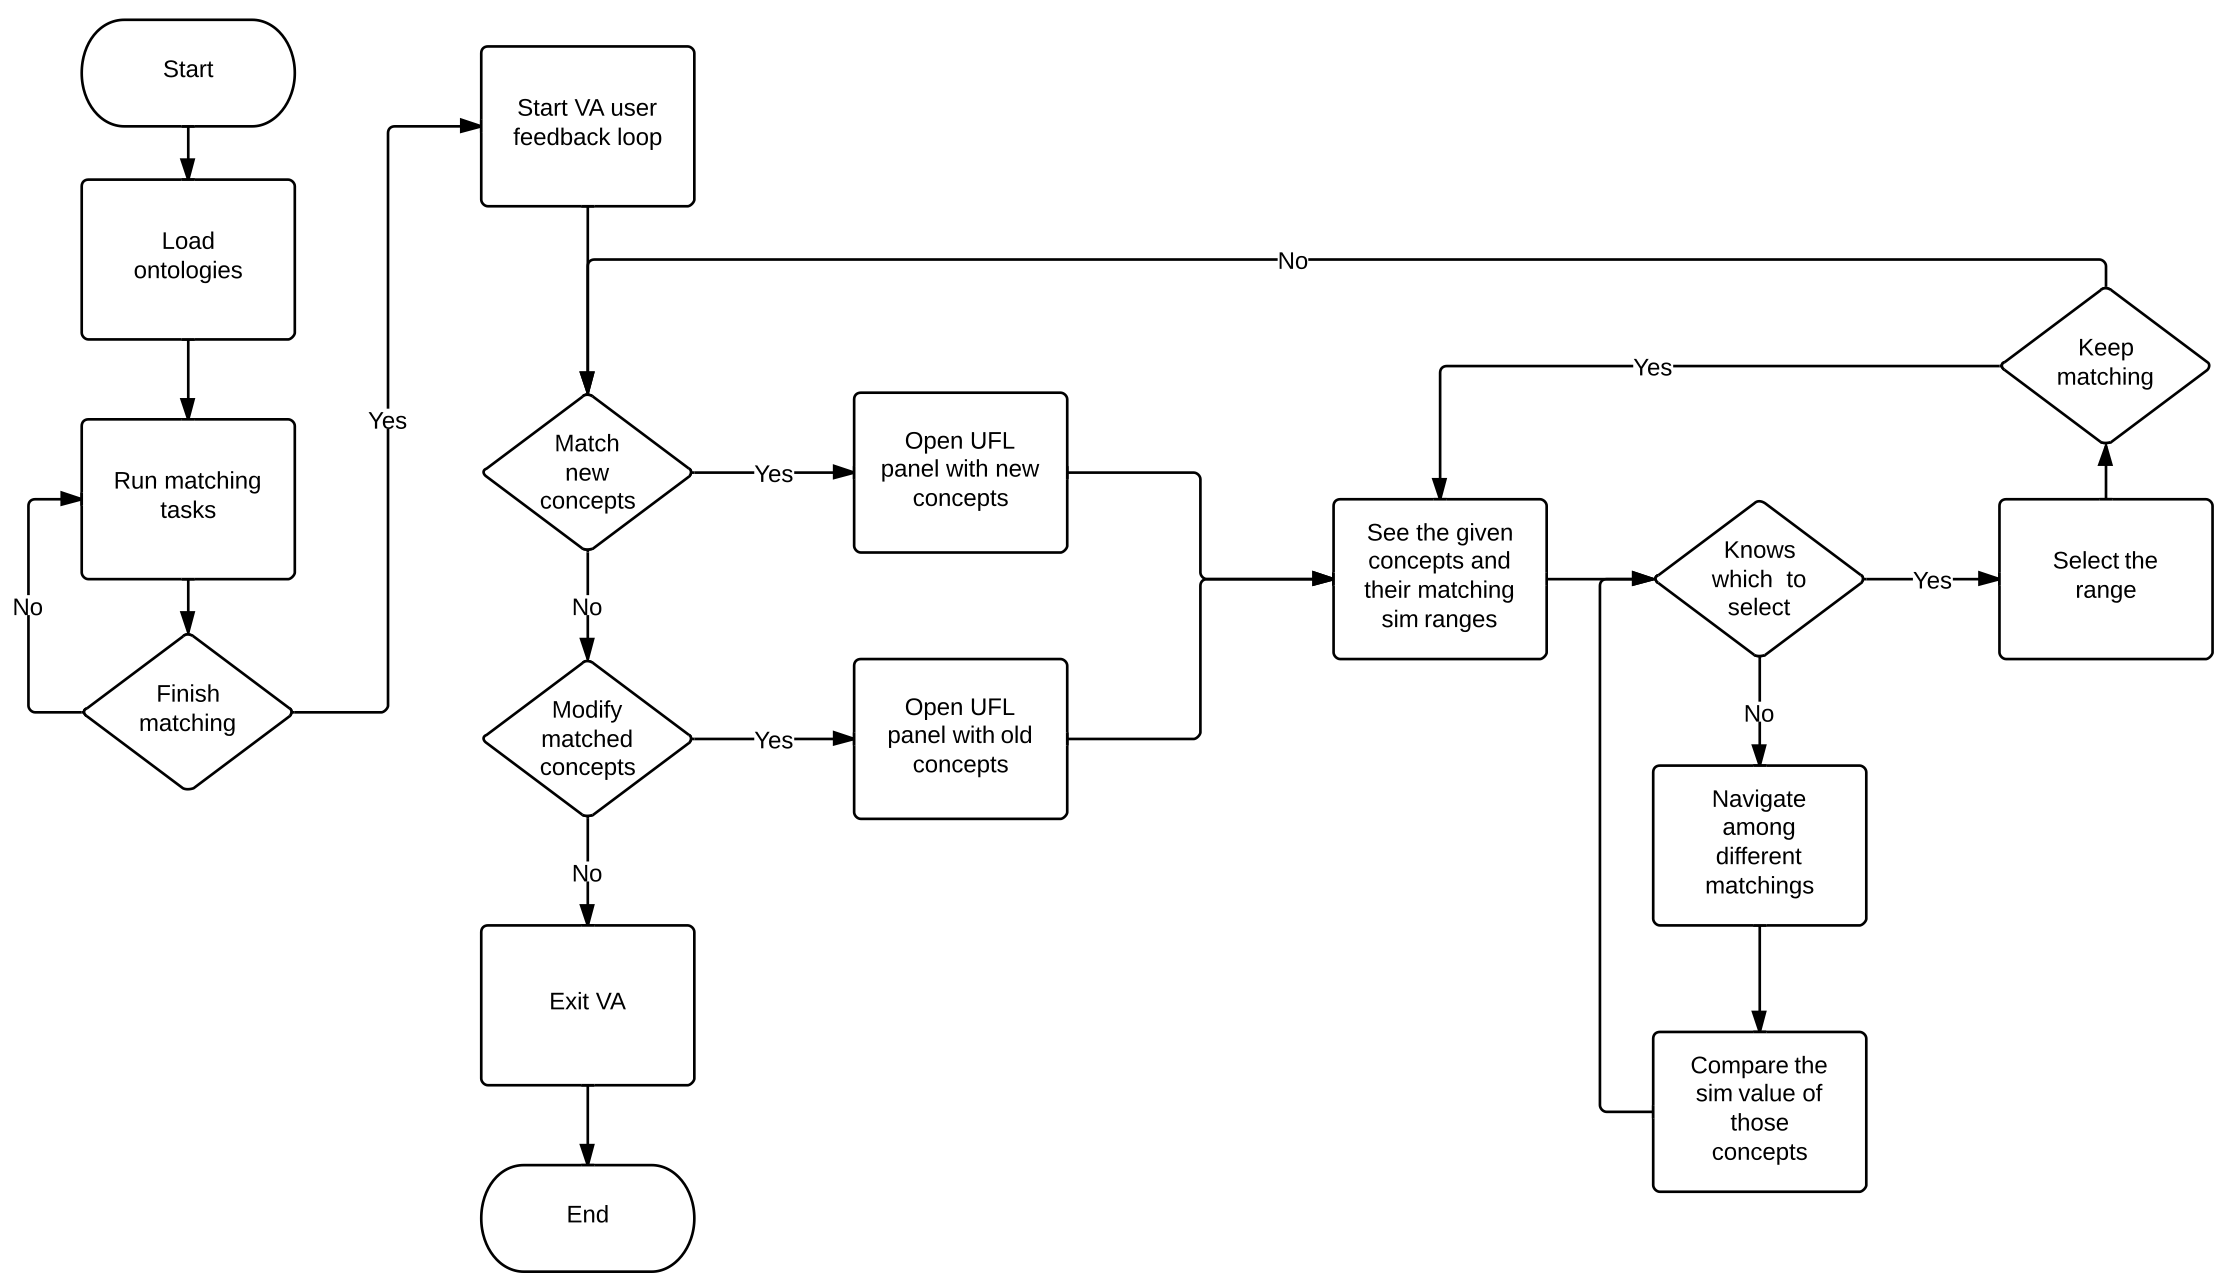
\includegraphics[width=6.5in]{pics/flow.png}
	\caption{Workflow}
	\label{fig:workflow}
\end{figure*}

%%=========================================
\section{Graphic User Interface}
We are making full use of the containers in JavaFx, in order to manage the elements within the limited space. See Fig.\ref{fig:ui} for the graphic user interface design. We use two tile panels to display two sets of ontology pairs, the upper panel is the main panel and the lower one is the sub panel (this will be talked in more detail in the next chapter). The treeview shows the siblings of the source ontology in the main panel and the listview shows the children nodes of a particular portion which user clicks on of the source ontology. 

\begin{figure*}[!ht]
	\centering
	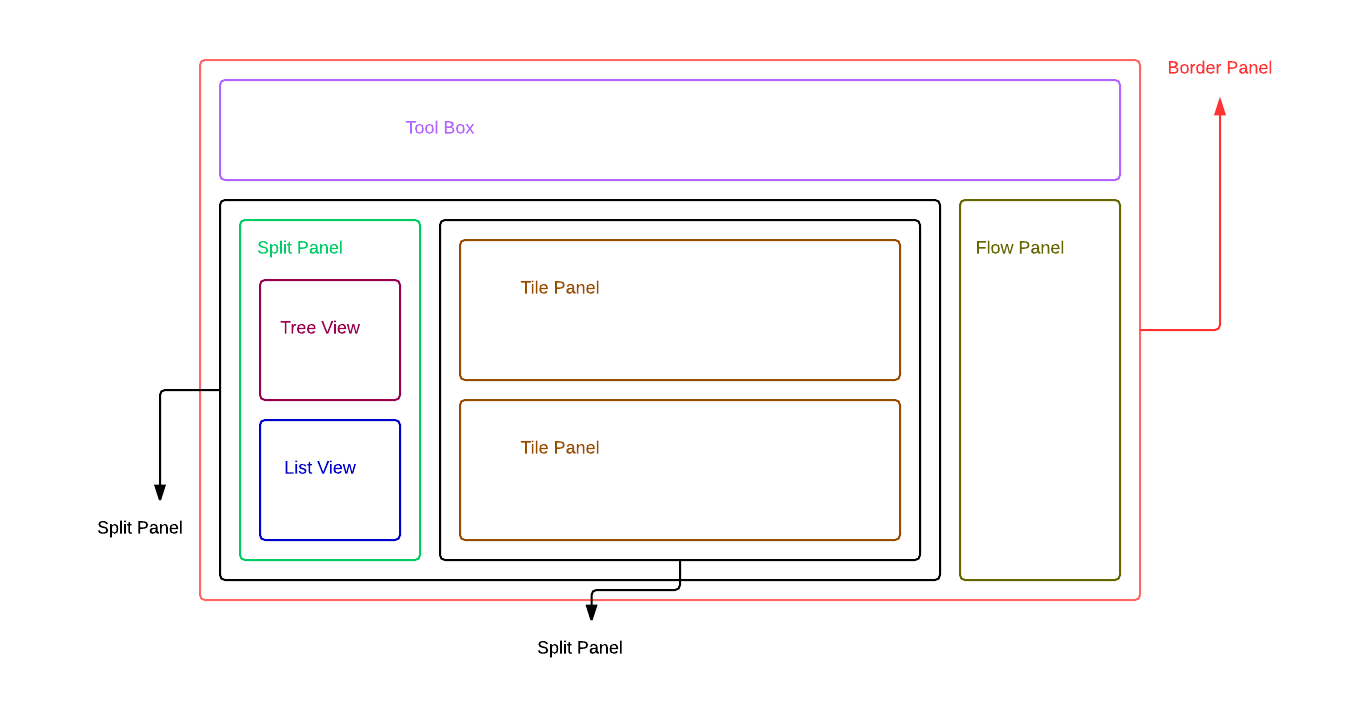
\includegraphics[width=6.5in]{pics/VA_UI.png}
	\caption{GUI}
	\label{fig:ui}
\end{figure*}
